\documentclass{beamer}
\usetheme{Antibes}
\usepackage{epstopdf}
\usepackage{tikz}
\usetikzlibrary{chains}

\title[Cyber Range]{Design and Developement of a Cyber Range}
% \subtitle{Using Beamer}
\author[A. Mocanu]{Alexandru Mocanu}
\institute[UniTo]{Università Degli Studi di Torino\\ Dipartimento di Informatica}
\date{\today}

\begin{document}


\begin{frame}
    \titlepage
\end{frame}

\begin{frame}
    \frametitle{Outline}

    \tableofcontents

\end{frame}

\section{Cyber Range}
\begin{frame}
    \frametitle{Cyber Range}

    È un ambiente virtuale usato da professionisti, e non, per testare:
    \begin{itemize}
        \item Affidabilità
        \item Sicurezza
        \item Prestazioni
    \end{itemize}
    di infrastrutture e sistemi IT.
\end{frame}

\section{CTF - Capture the Flag}
\begin{frame}
    \frametitle{CTF - Capture the Flag}

    È un gioco di \textbf{hacking} dove team (o singoli) cercano \textbf{vulnerabilità} in sistemi
    e software messi a disposizione dagli organizzatori della competizione al fine di sfruttarle e 
    di collezionare le varie \textbf{flag} nascoste sul sistema bersaglio.
    

\end{frame}
\subsection{Tipologie CTF}
\begin{frame}
    \frametitle{Tipologie CTF}
    Ci sono vari tipi di Capture the Flag, i più famosi sono:
    \begin{itemize}
        \item Jeopardy
        \item Attack/Defense
        \item Boot2Root
    \end{itemize}
    

\end{frame}

\begin{frame}
    \frametitle{CTF - Jeopardy}
    I CTF di tipo Jeopardy sono probabilmente i più popolari, dato che si adattano bene a competizioni online.
    \\
    In questo formato:
    \begin{itemize}
        \item<1-> diverse \textit{challenge}, ognuna con un singolo \textit{flag}
        \item<2-> \textbf{punteggio}: a seconda della difficoltà della singola \textit{challenge}
        \item<3-> \textbf{vincitore}: chi totalizza il punteggio maggiore
        \item<4-> \textbf{durata}: a tempo
    \end{itemize}

    \onslide<5->{Generalmente con questo tipo di formato i partecipanti formano squadre,
    le quali assegnano una challenge a uno o più membri della squadra, per velocizzare 
    la risoluzione delle challenge e la conquista delle flag.}
    
    

\end{frame}

\begin{frame}
    \frametitle{CTF - Attack/Defense}
    Il formato Attack/Defense prevede che gli organizzatori 
    forniscano ai giocatori (principalmente squadre) una o più macchine virtuali.
    \\~\\
    \onslide<2->{I giocatori quindi avranno un doppio ruolo:}
    \begin{itemize}
        \item <3->\textbf{difendere} i servizi esposti sulla propria macchina virtuale
        \item <4->\textbf{attaccare} i servizi dei team concorrenti
    \end{itemize}
    \leavevmode \\~\\
    \onslide<5->{Si guadagna un \textbf{punteggio} per ogni flag conquistato.}
    \\~\\
    \onslide<6->{Generalmente sono eventi \textit{offline} e con un limite di tempo.}

\end{frame}

\begin{frame}
    \frametitle{CTF - Boot2Root}
    Consiste l'installazione di una \textit{macchina virtuale} e lo scopo è di trovare e sfruttarne le
    vulnerabilità che permettano di avere l'accetto root alla stessa.
    \\~\\
    \onslide<2->{Questo formato di CTF è principalmente preferito da singoli 
    che vogliono esercitarsi a sfruttare vulnerabilità in uno scenario 
    semi-reale, ma non preclude la possibilità di creare un team.}

\end{frame}



\section{Scenario immaginato}

\begin{frame}
    \frametitle{Scenario}

    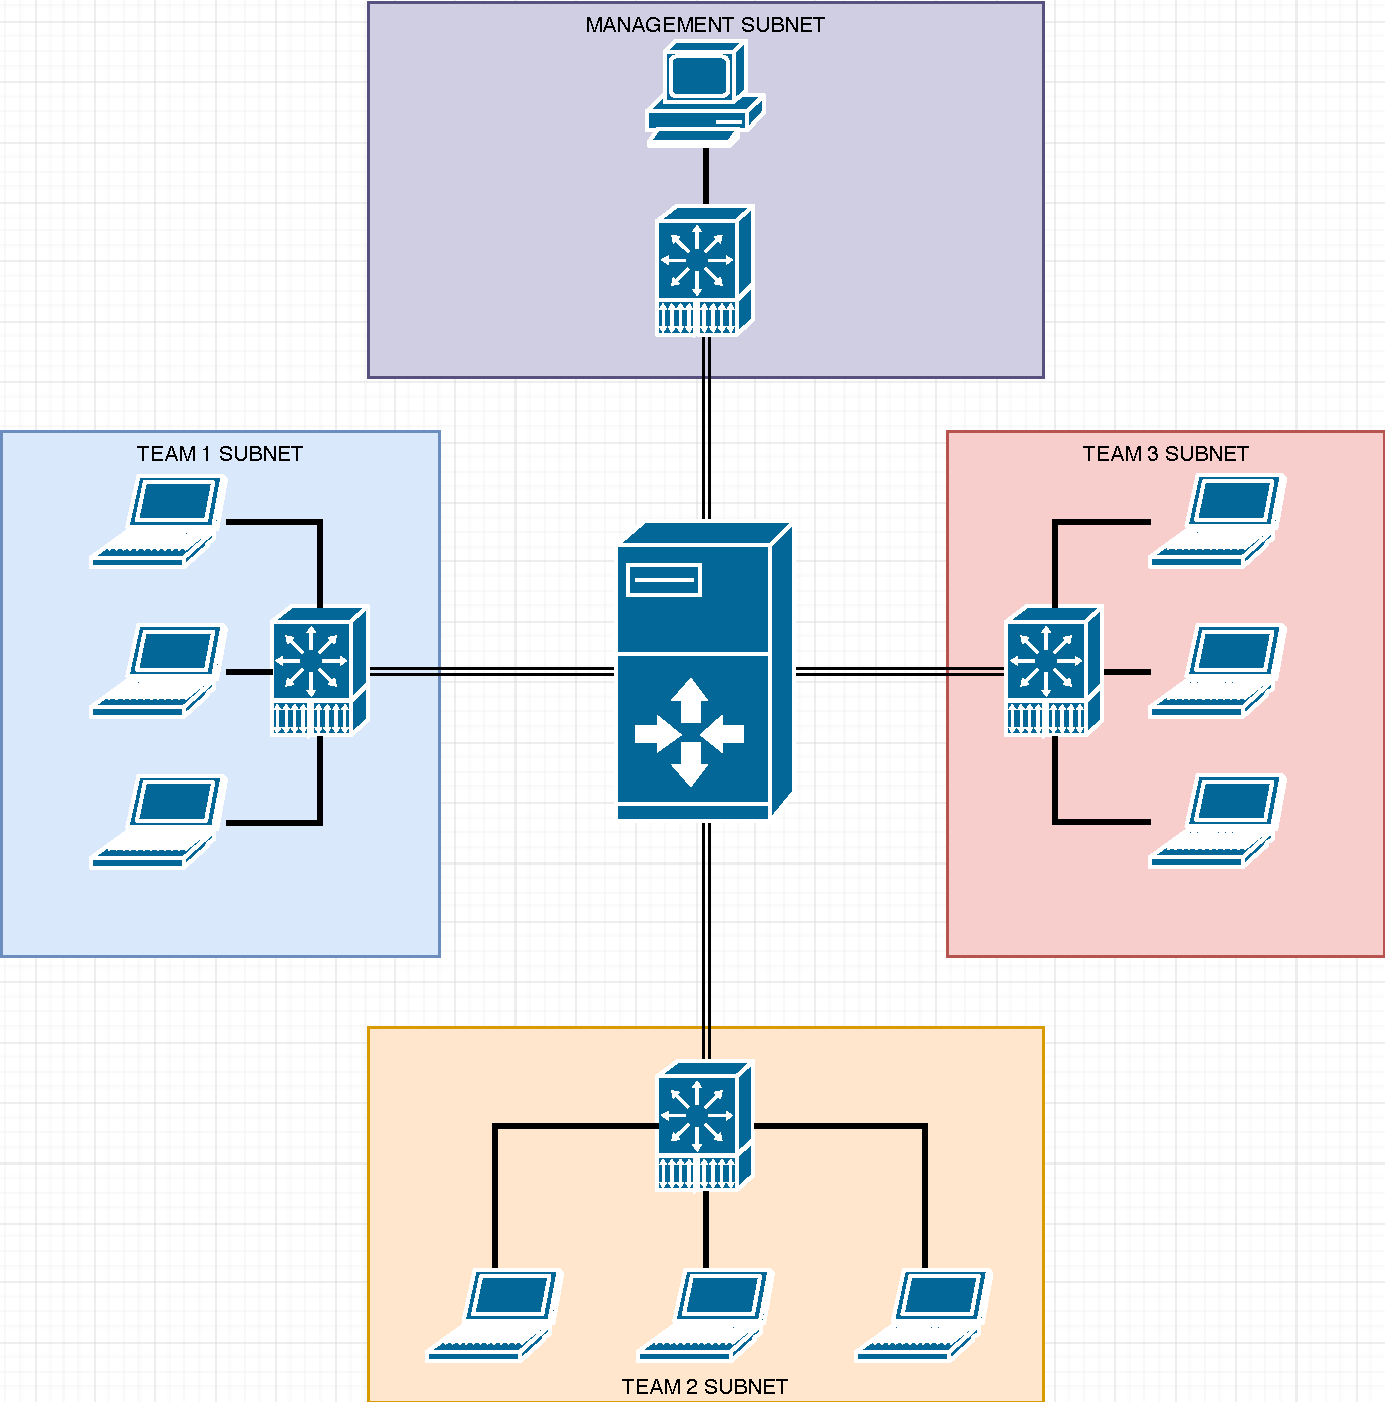
\includegraphics[width=\textwidth]{competition.pdf}

\end{frame}

\section{Regole Firewall}




\subsection{Fase 1}
\subsubsection{Obiettivi}
\begin{frame}
    \frametitle{Obiettivi Fase 1}


\end{frame}

\subsubsection{Regole specifiche per il Virtual Router}
\begin{frame}
    \frametitle{Regole specifiche per il Virtual Router}
    \begin{itemize}
        \item aa
    \end{itemize}
\end{frame}


\subsubsection{Regole specifiche per il Management}
\begin{frame}
    \frametitle{Regole specifiche per il Management}
    \begin{itemize}
        \item aaa
    \end{itemize}

\end{frame}

\subsubsection{Regole specifiche per i Team}
\begin{frame}
    \frametitle{Regole specifiche per i Team}
    \begin{itemize}
        \item aaa
    \end{itemize}

\end{frame}

\subsection{Fase 2}
\subsubsection{Obiettivi}
\begin{frame}
    \frametitle{Obiettivi Fase 2}

    

\end{frame}
\subsubsection{Regole specifiche per il Virtual Router}
\begin{frame}
    \frametitle{Regole specifiche per il Virtual Router}
    \begin{itemize}
        \item aa
    \end{itemize}
\end{frame}


\subsubsection{Regole specifiche per il Management}
\begin{frame}
    \frametitle{Regole specifiche per il Management}
    \begin{itemize}
        \item aa
    \end{itemize}

\end{frame}

\subsubsection{Regole specifiche per i Team}
\begin{frame}
    \frametitle{Regole specifiche per i Team}
    \begin{itemize}
        \item aa
    \end{itemize}

\end{frame}


\section{Tools \& Software}
\begin{frame}
    \frametitle{Software}
    \begin{itemize}
        \item <1-> iptables
        \item <1-> netplan
        \item <1-> python
    \end{itemize}
     
\end{frame}

\section{Test delle prestazioni}
\begin{frame}
    \frametitle{}

    

\end{frame}


\end{document}


